\newpage 
\section{2 lepton ATLAS data analysis}

The 3 lepton + $e_T^{miss}$ dataset has less events, and thus allows for less training of the neural networks. 
Thus, the 2 lepton + $e_T^{miss}$ dataset was tried instead. The event selection was done choosing atleast 
2 leptons, meaning that the RMM signatures of some of the events will look similar to the RMM signatures of 
the 3 lepton + $e_T^{miss}$ dataset. A consequence of this is that the signal samples for the 3 lepton case 
would be a good start point for testing. The signal region for the regular autoencoder models were created by 
calculating the median $m_{err}$ of the reconstruction error. Then, 3 cuts were made, starting at 
$m_{err} + im_{err}/5$ for $i = 1,2,3$. As the shape of the background reconstruction error has a hill like 
shape, the median is a good place to start to remove alot of the background. This is however just a guess 
for an optimal signal region, as the true signal is unknown, and the method has to be as unbiased as possible. 
Below are some of the results from training on the 2 lepton case, using the same two SUSY signals as test cases. 


\begin{figure}
    \centering
    \begin{subfigure}{.45\textwidth}
        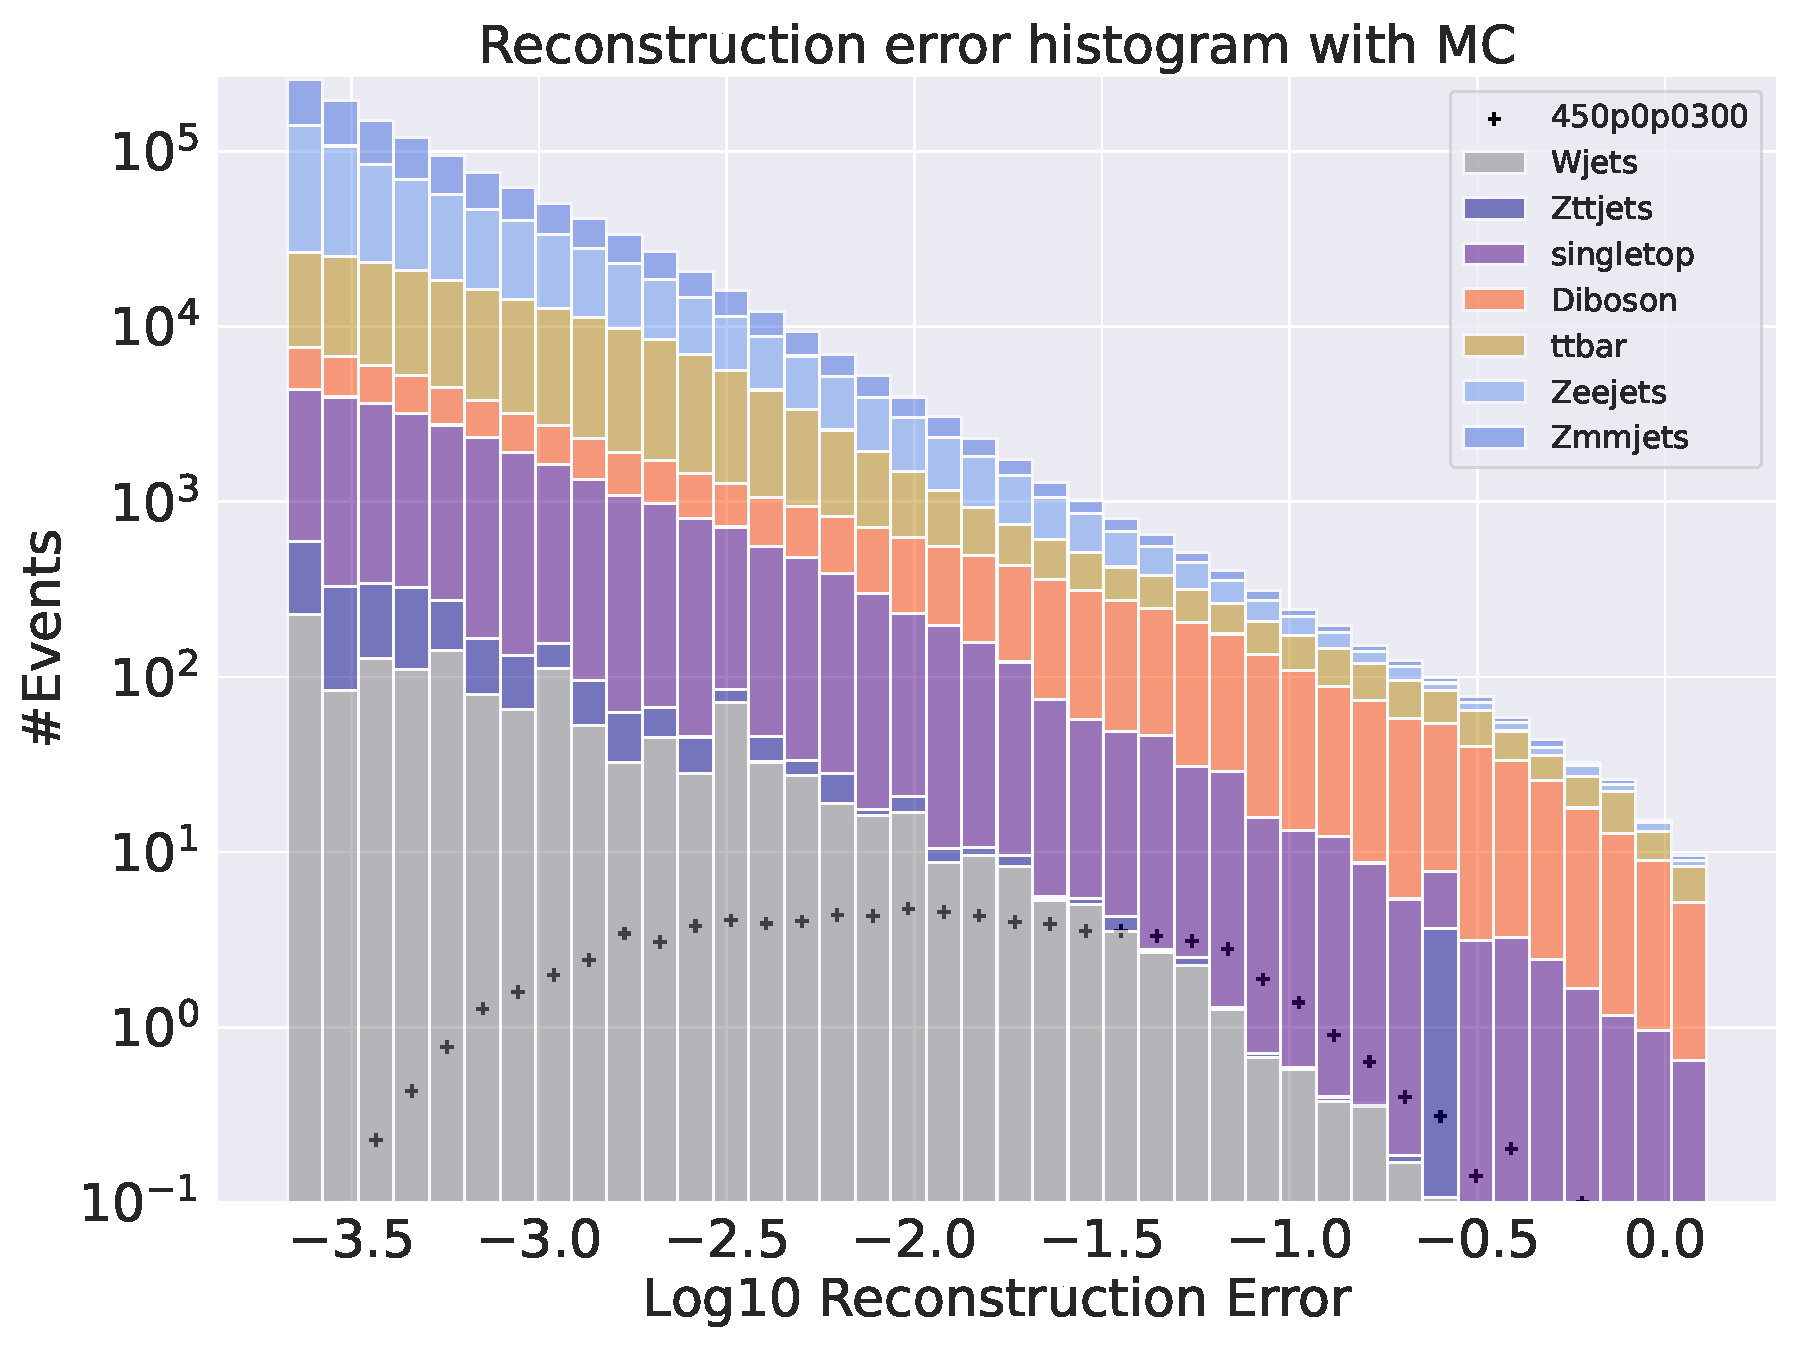
\includegraphics[width=\textwidth]{Figures/AE_testing/big/2lep/b_data_recon_big_rm3_feats_sig_450p0p0300_.pdf}
        \caption{ }
        \label{fig:AE_2lep_big_450}
    \end{subfigure}
    \hfill
    \begin{subfigure}{.45\textwidth}
        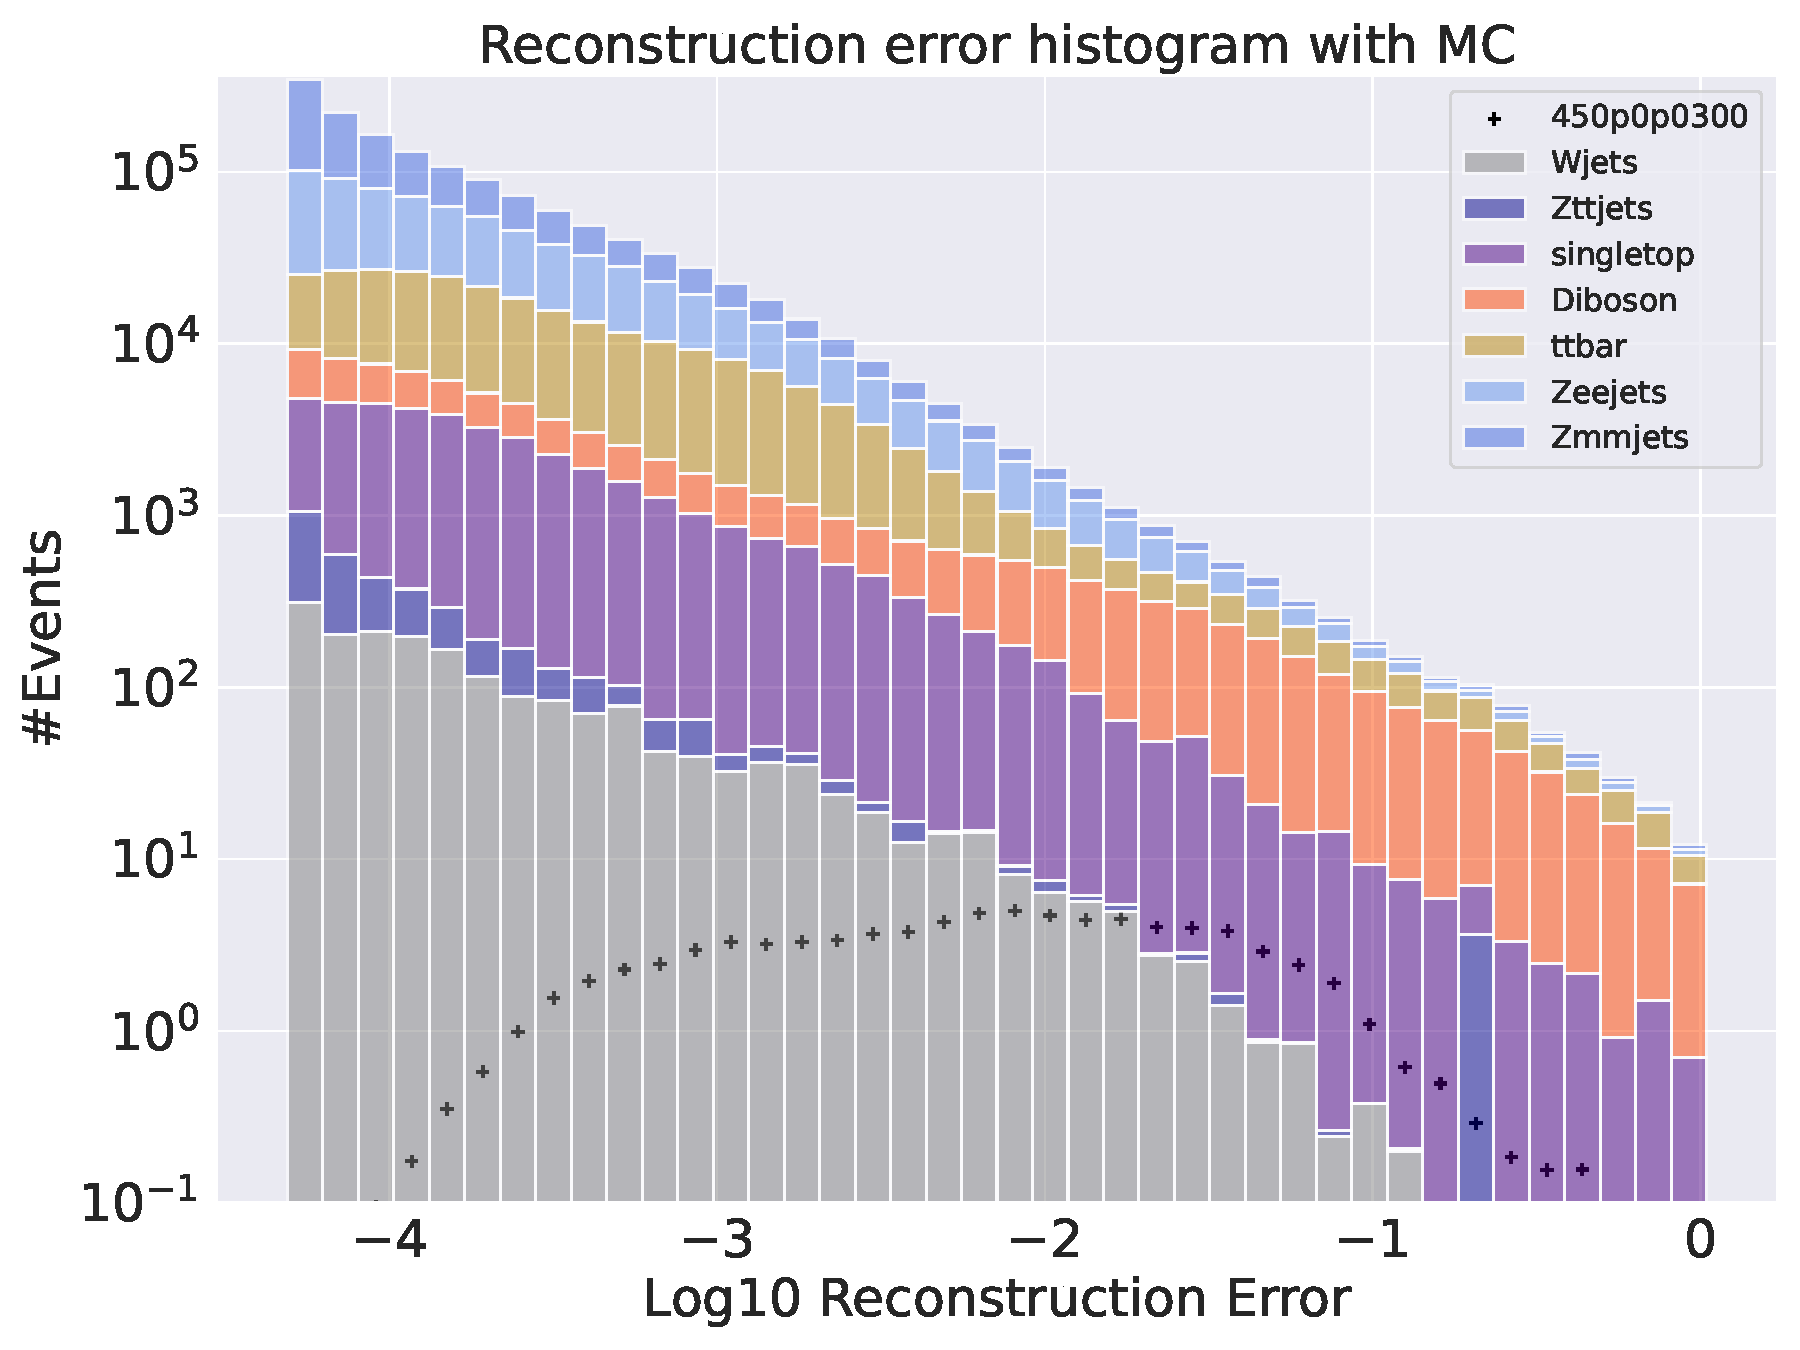
\includegraphics[width=\textwidth]{Figures/AE_testing/small/2lep/b_data_recon_big_rm3_feats_sig_450p0p0300_.pdf}
        \caption{}
        \label{fig:AE_2lep_small_450}
    \end{subfigure}
    \hfill
    \begin{subfigure}{.45\textwidth}
        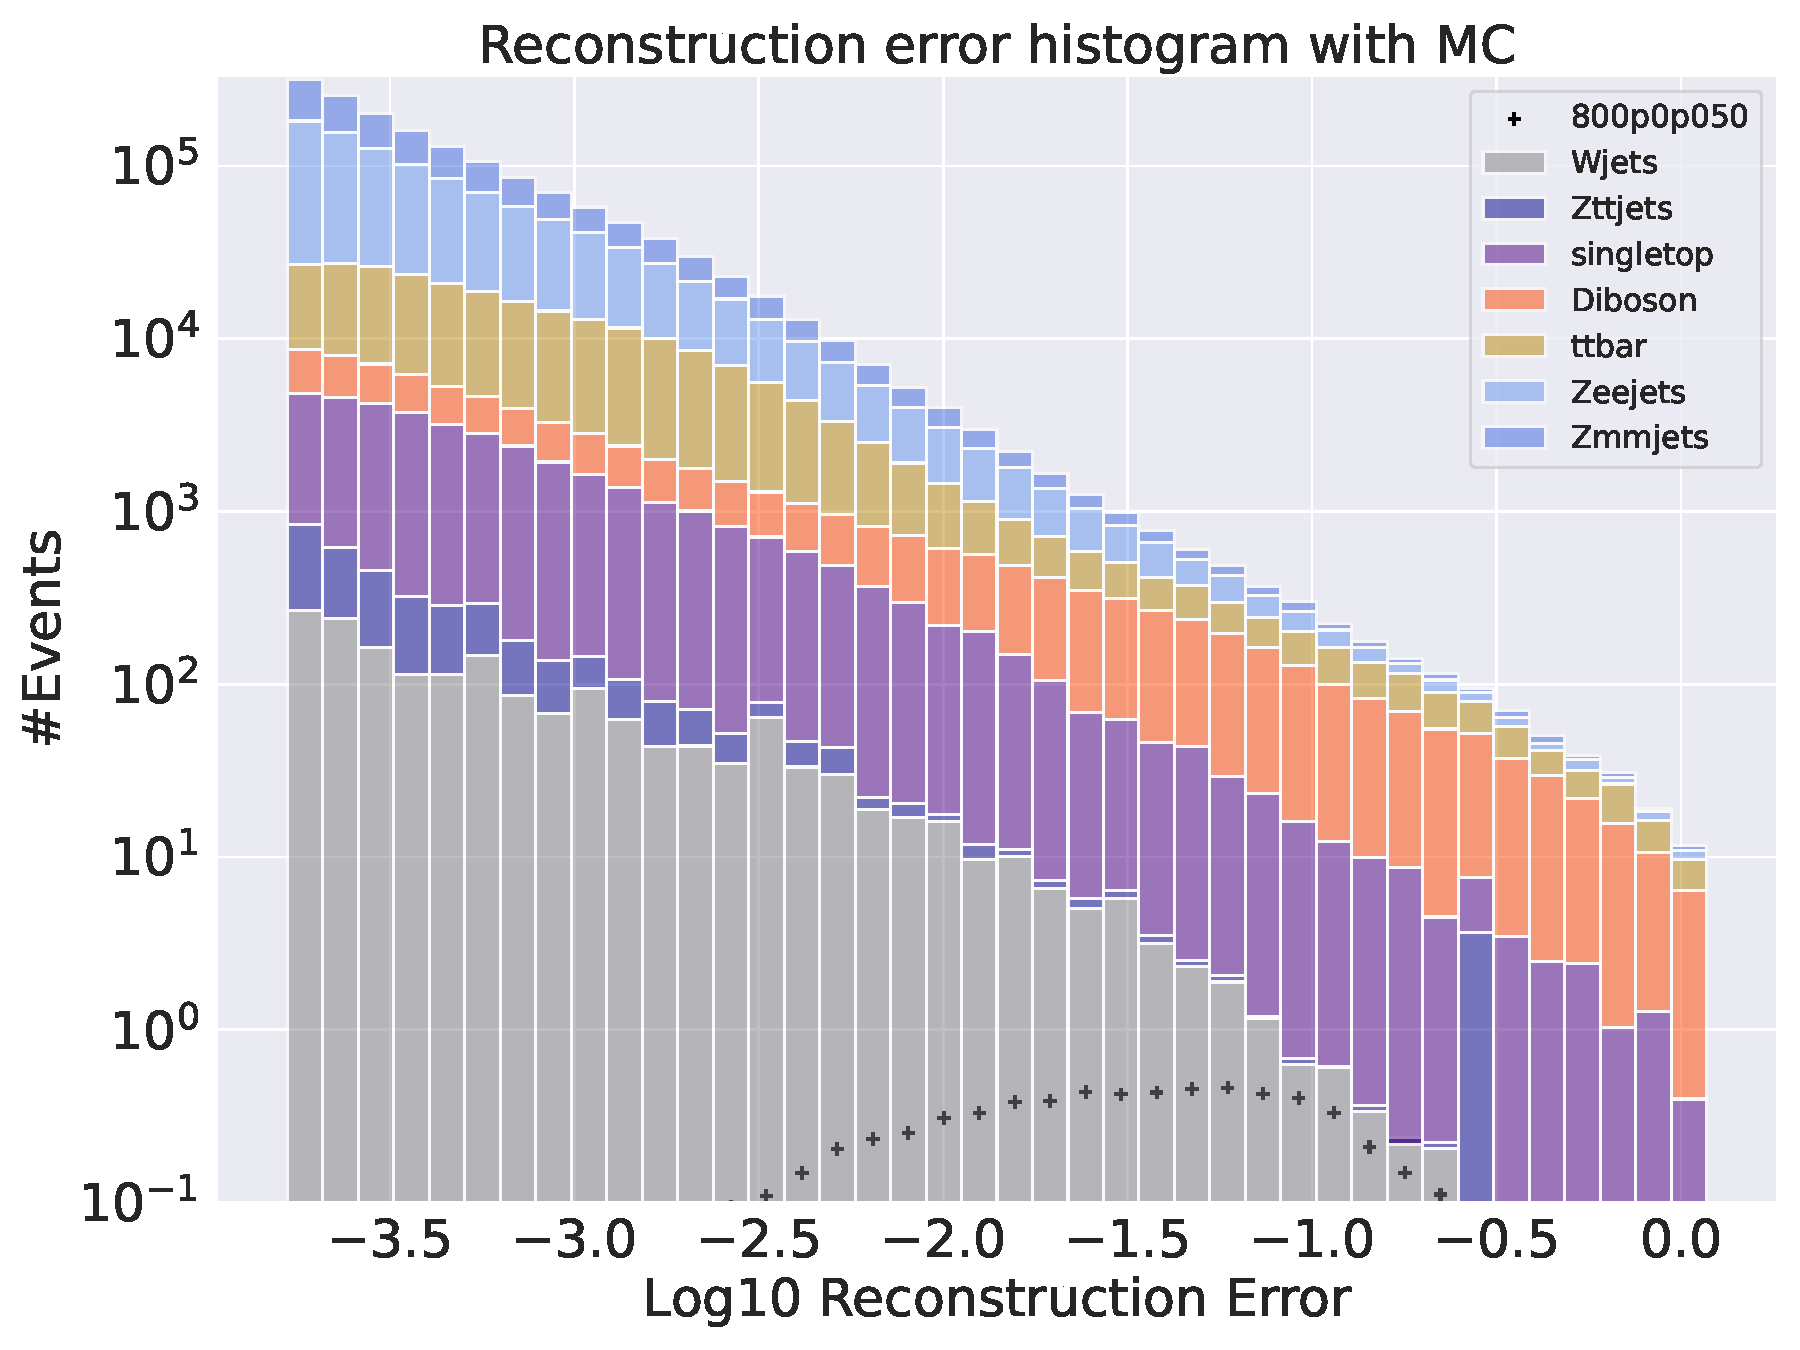
\includegraphics[width=\textwidth]{Figures/AE_testing/big/2lep/b_data_recon_big_rm3_feats_sig_800p0p050_.pdf}
        \caption{}
        \label{fig:AE_2lep_big_800}
    \end{subfigure}
    \hfill   
    \begin{subfigure}{.45\textwidth}
        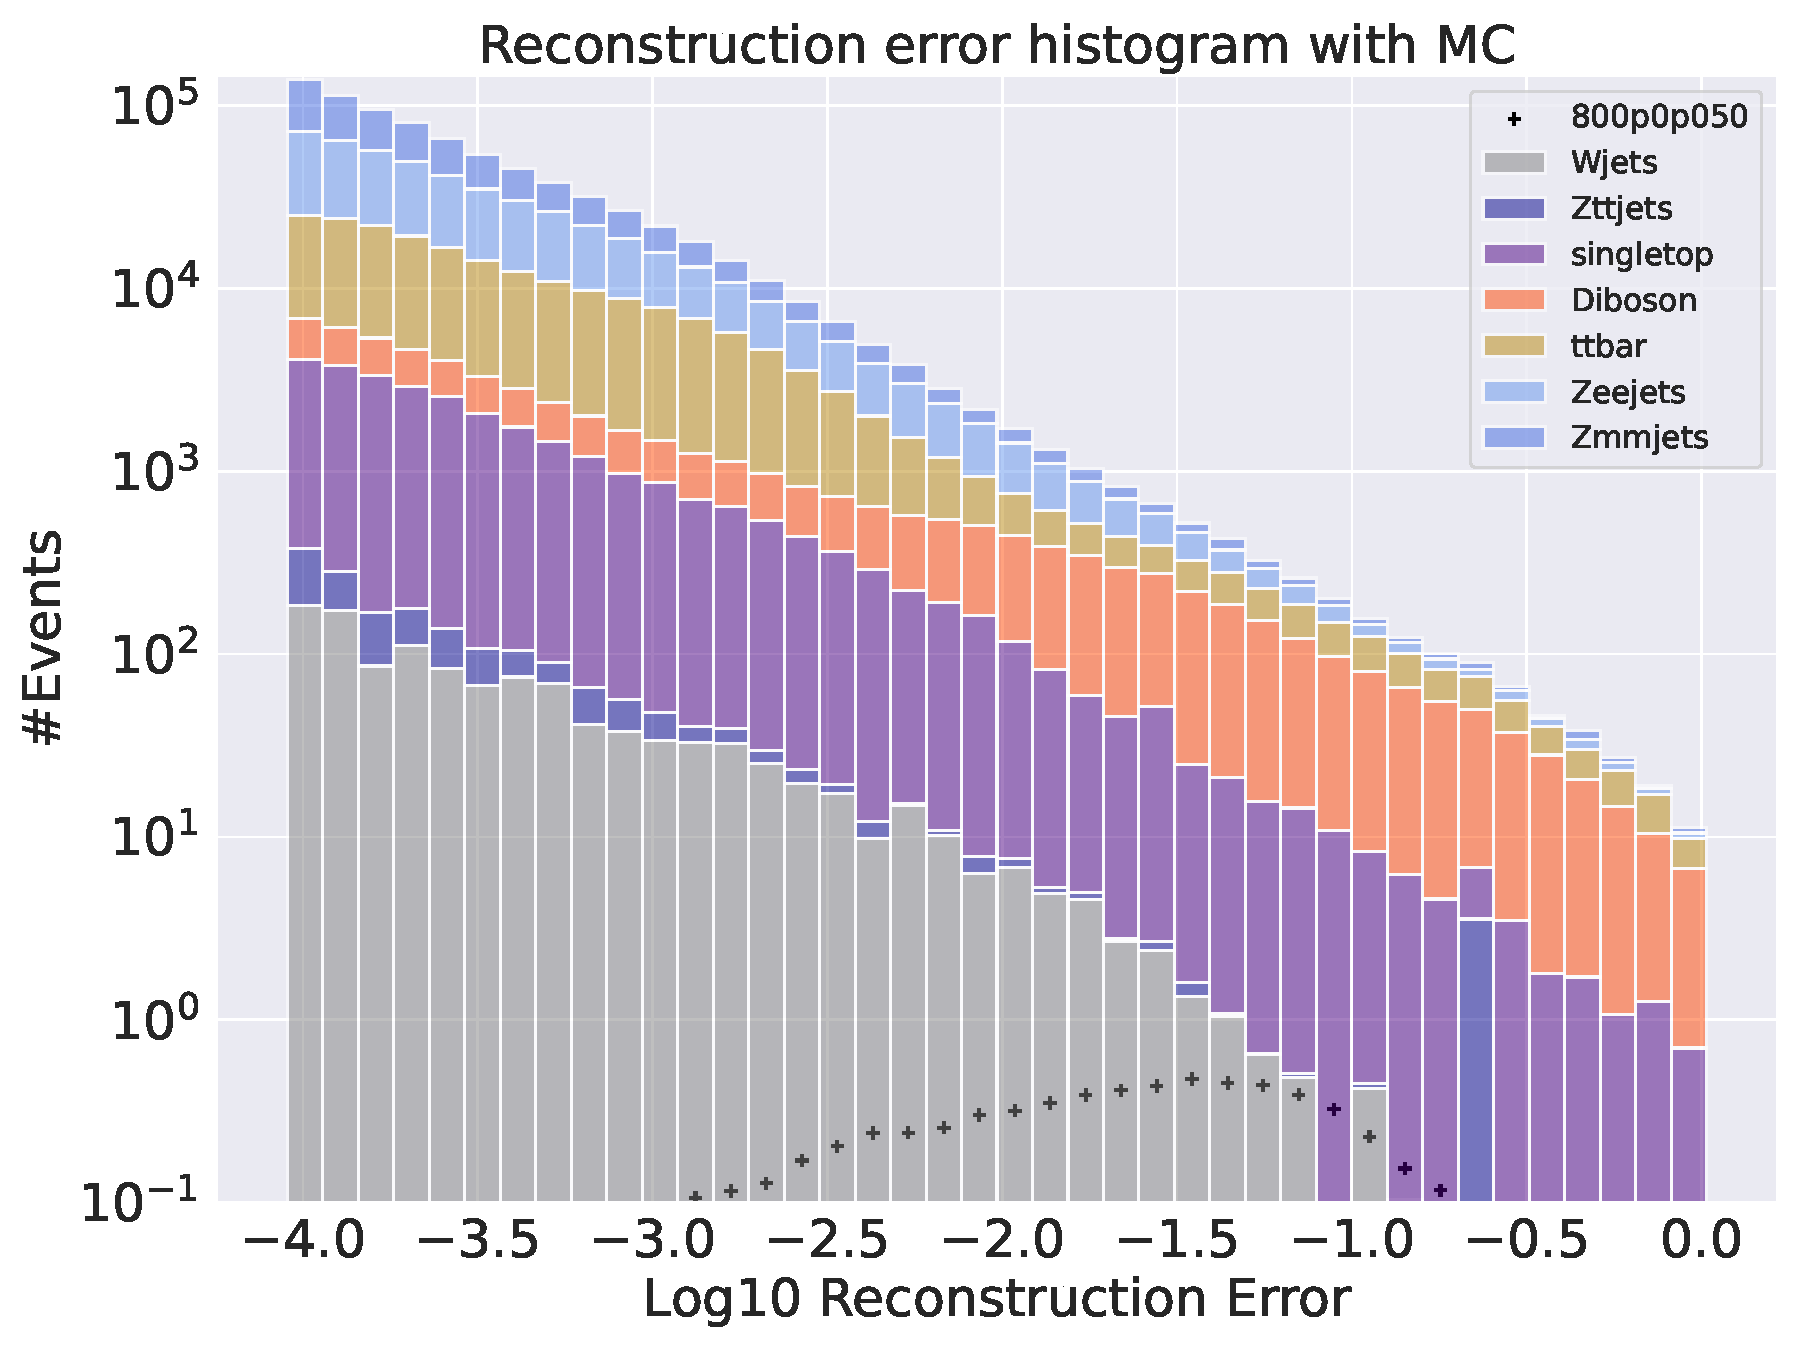
\includegraphics[width=\textwidth]{Figures/AE_testing/small/2lep/b_data_recon_big_rm3_feats_sig_800p0p050_.pdf}
        \caption{}
        \label{fig:AE_2lep_small_800}
    \end{subfigure}
    \hfill      
    \caption[2lep reconstruction error with SUSY signals]{Reconstruction error distribution for the small (left) and large (right)
    regular autoencoder, using the 2 lepton + $e_T^{miss}$ dataset as training and test set. The signals used are the same SUSY signals 
    from the 3 lepton case. Figures \ref{fig:AE_2lep_big_450} and \ref{fig:AE_2lep_small_450} shows the SUSY 450 and 300 mass signal, 
    and figures \ref{fig:AE_2lep_big_800} and \ref{fig:AE_2lep_small_800} shows the SUSY 800 and 50 mass signal.}
    \label{fig:AE_2lep_recon_err_both_sig}
\end{figure}

In figure \ref{fig:AE_2lep_recon_err_both_sig} we have the reconstruction error distributions for the 2 lepton + $e_T^{miss}$ 
dataset for the regular autoencoder models. \par 
Using the signal region definition from above we set cuts on the reconstruction error and then calculate the significance of the signal. 
The figures with the best significance are shown below:

\begin{figure}
    \centering
    \begin{subfigure}{.45\textwidth}
        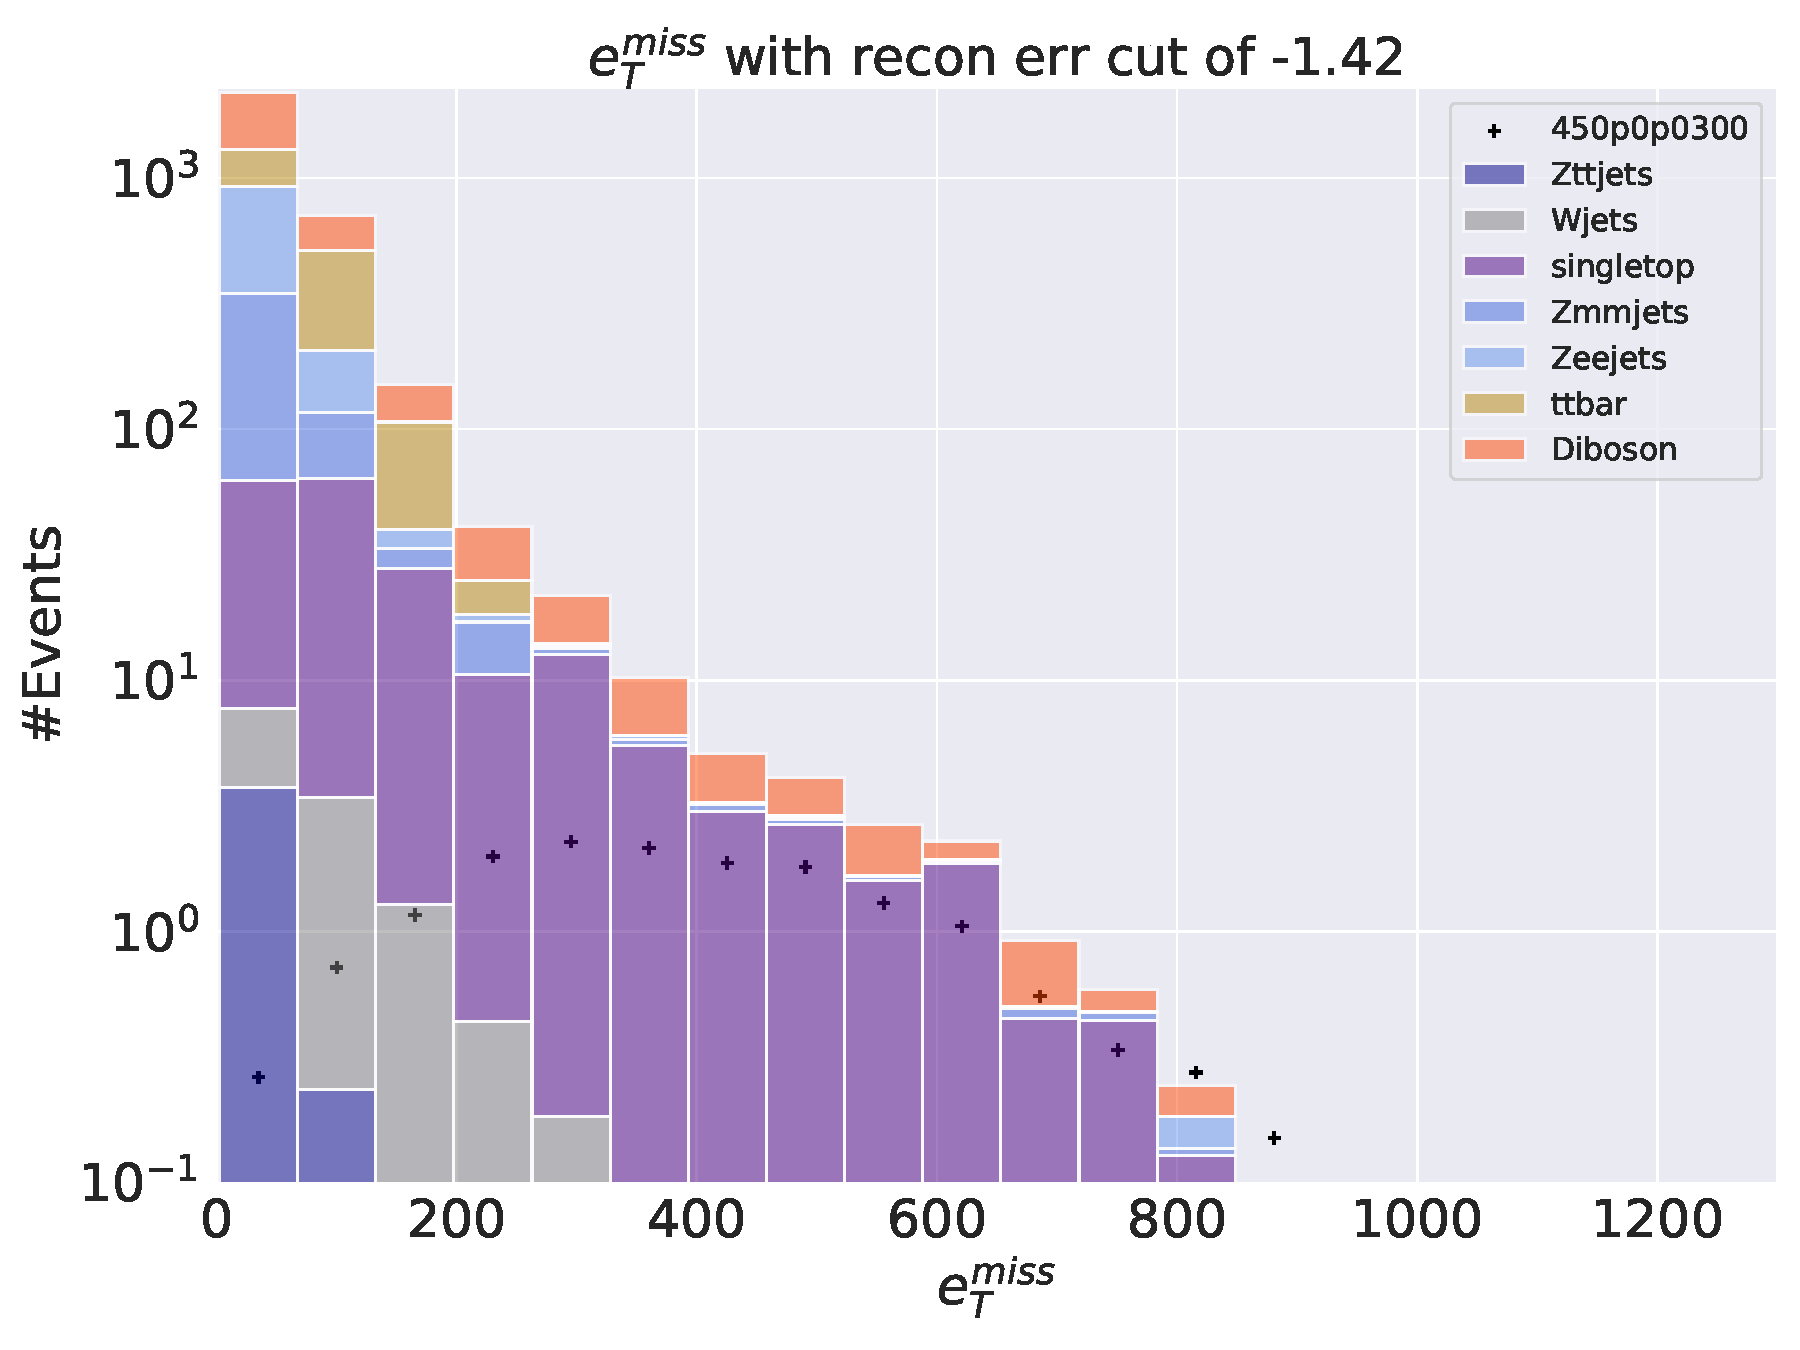
\includegraphics[width=\textwidth]{Figures/AE_testing/big/2lep/b_data_recon_big_rm3_feats_sig_450p0p0300_recon_errcut_-1.42.pdf}
        \caption{ }
        \label{fig:AE_2lep_big_450_cut_etmiss}
    \end{subfigure}
    \hfill
    \begin{subfigure}{.45\textwidth}
        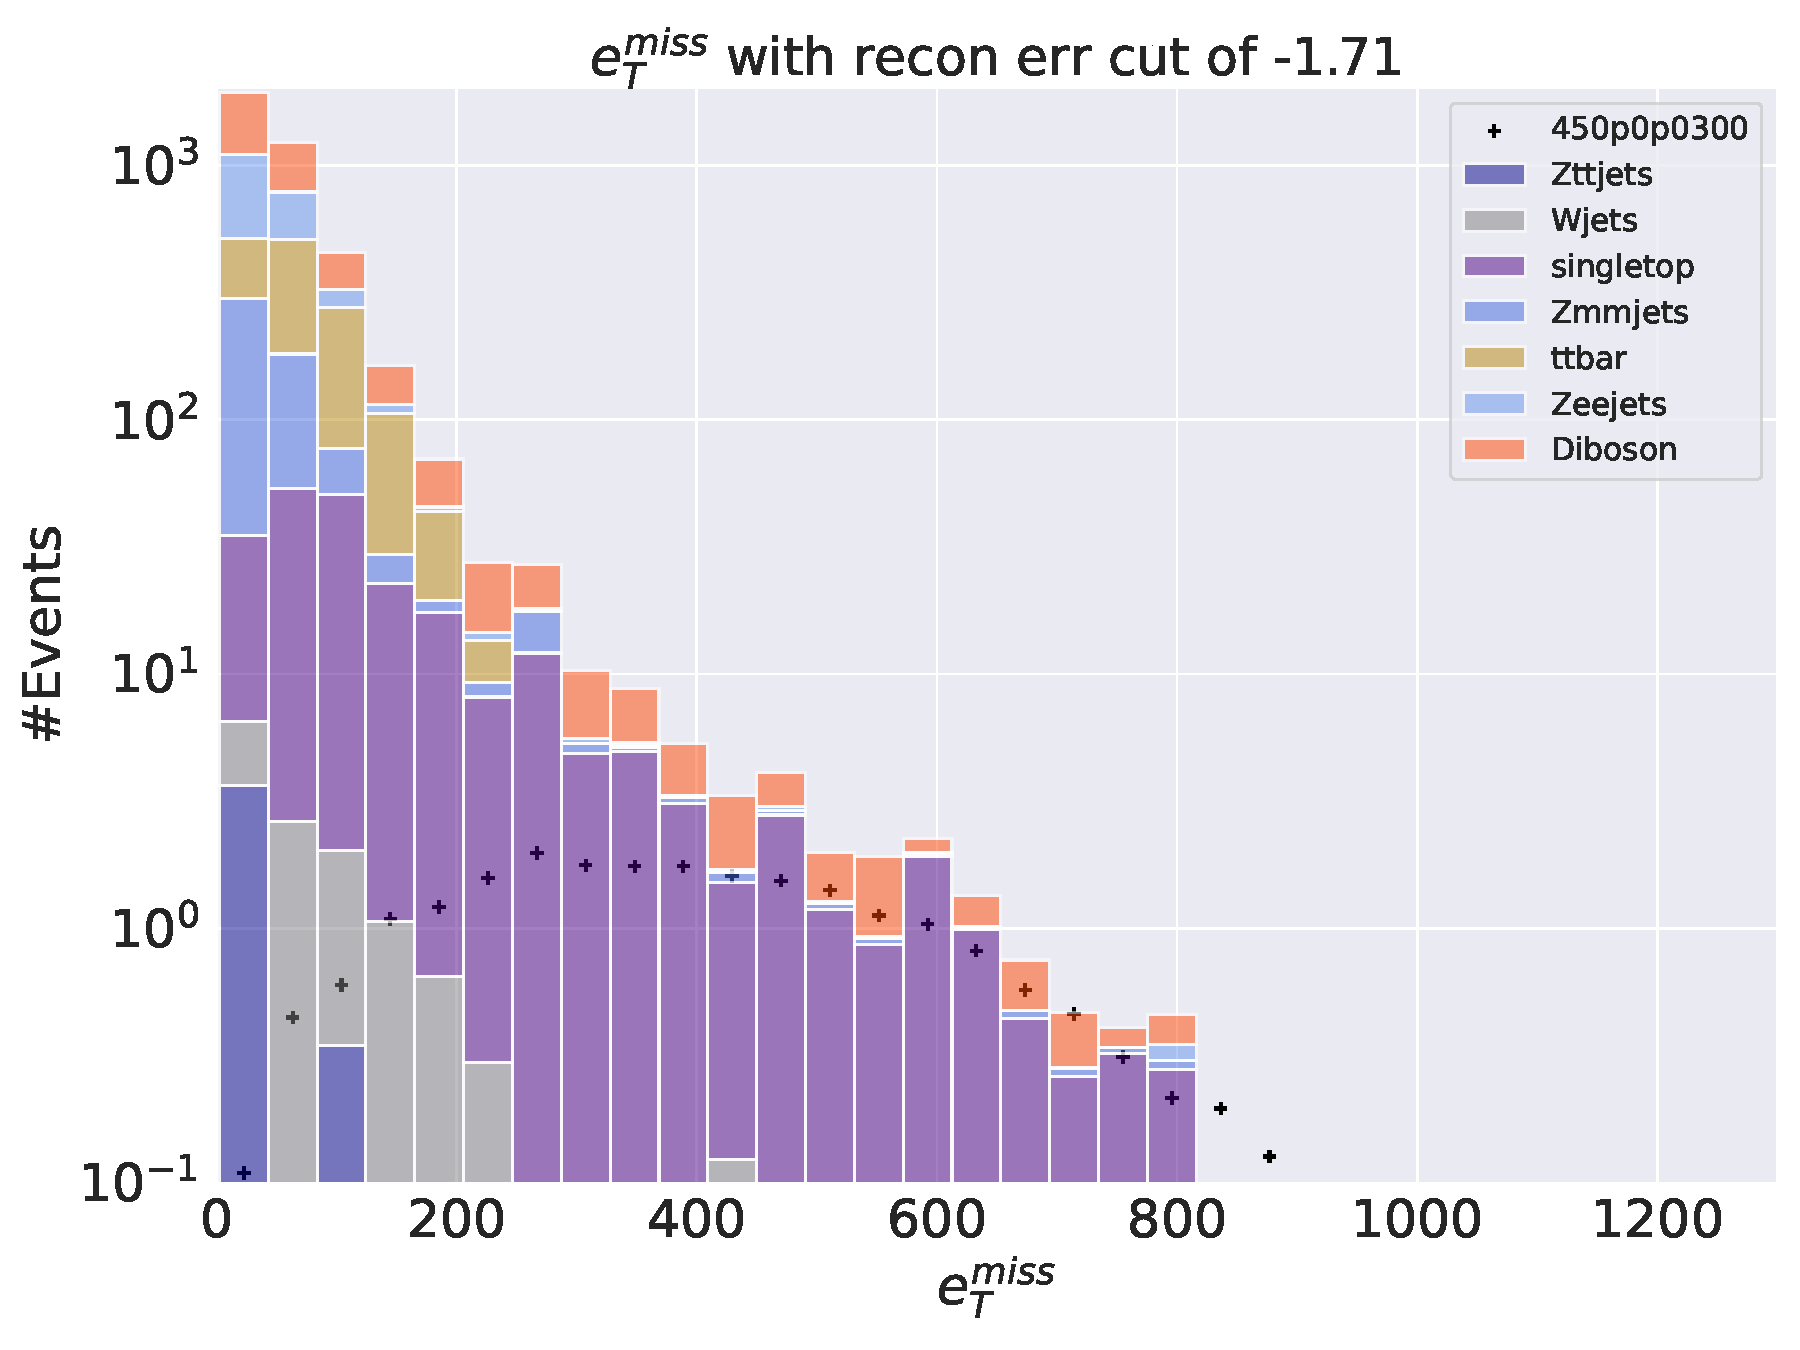
\includegraphics[width=\textwidth]{Figures/AE_testing/small/2lep/b_data_recon_big_rm3_feats_sig_450p0p0300_recon_errcut_-1.71.pdf}
        \caption{}
        \label{fig:AE_2lep_small_450_cut_etmiss}
    \end{subfigure}
    \hfill
    \begin{subfigure}{.45\textwidth}
        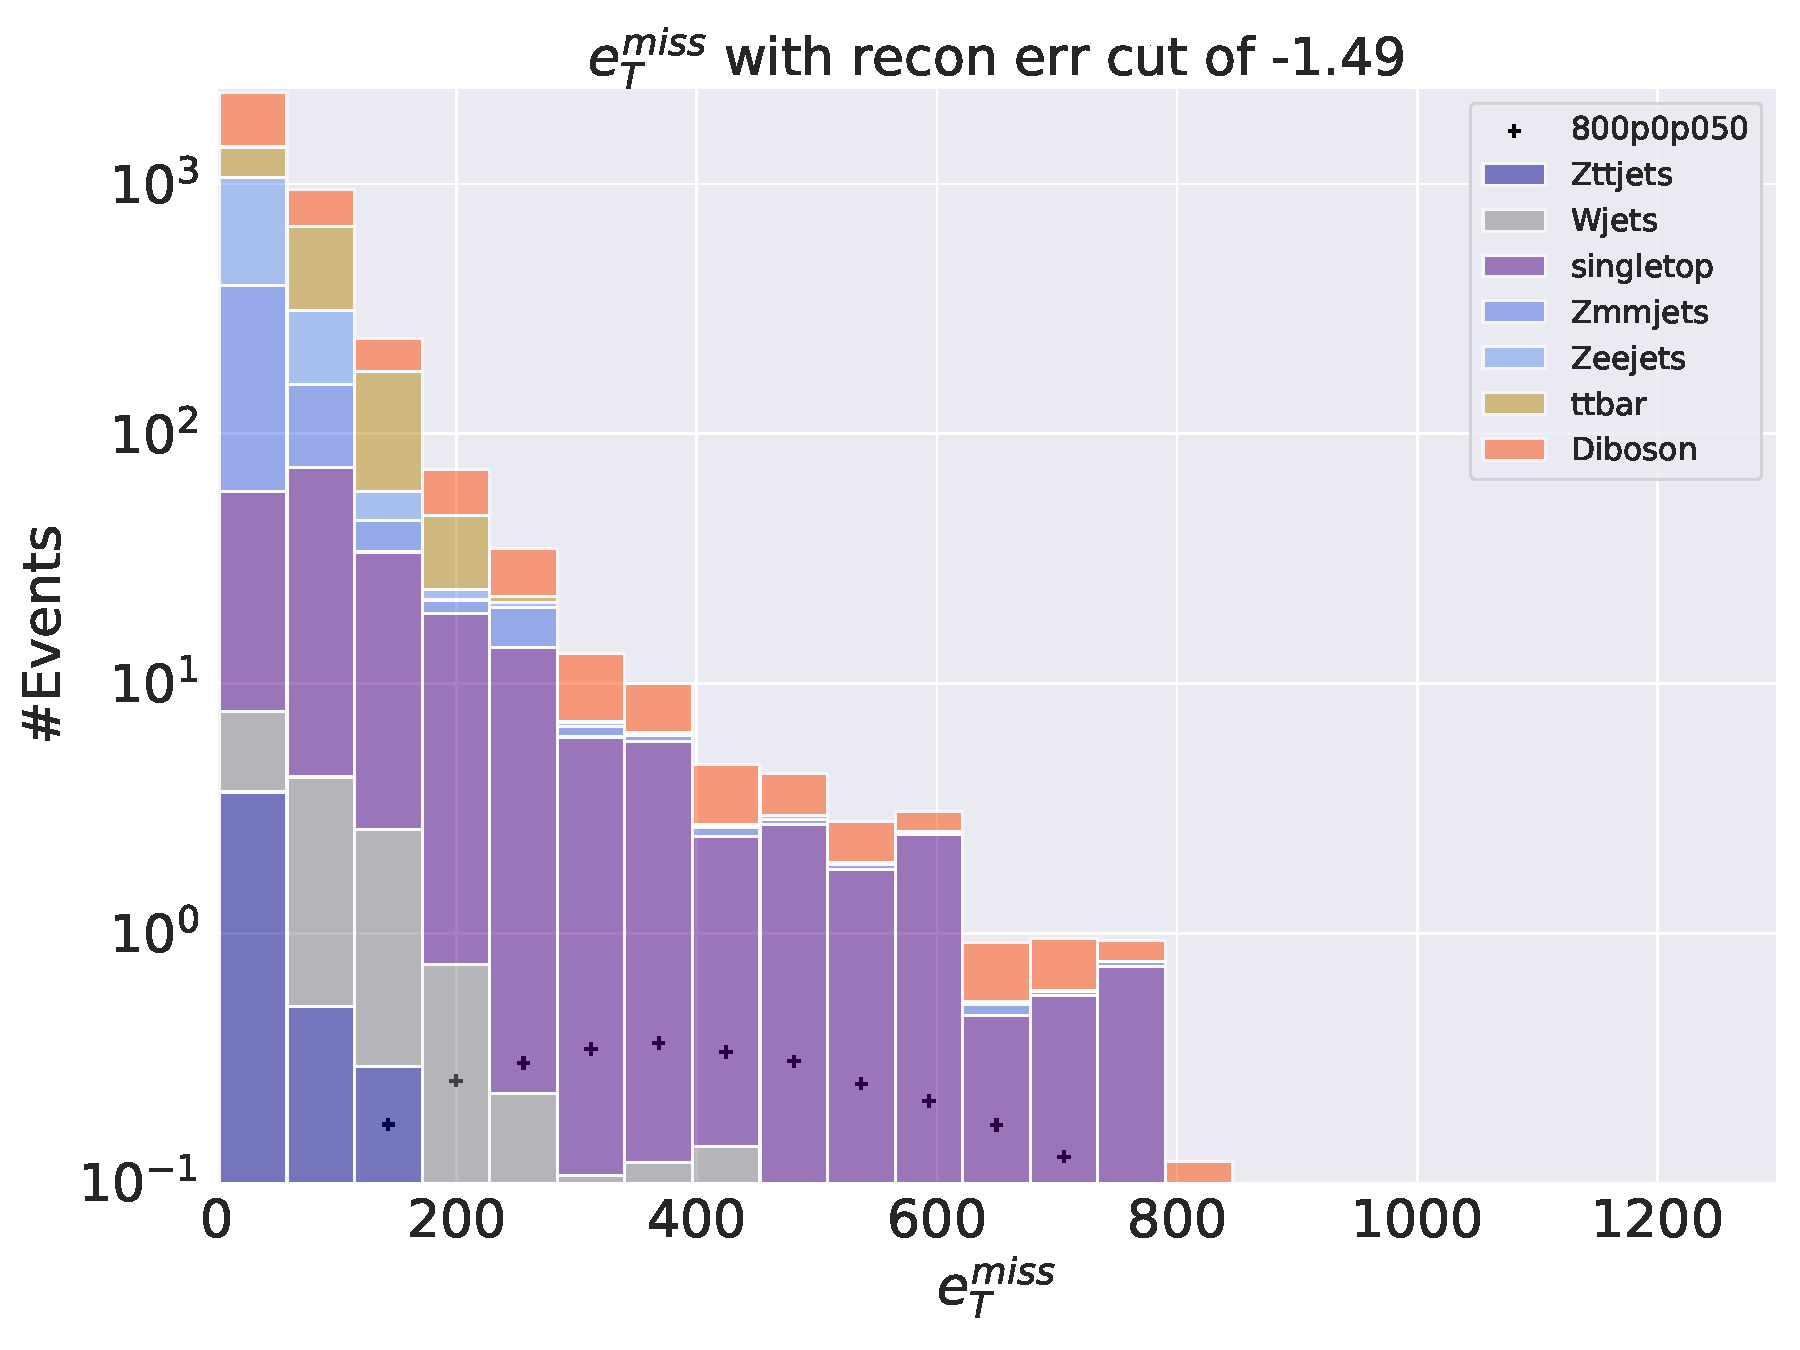
\includegraphics[width=\textwidth]{Figures/AE_testing/big/2lep/b_data_recon_big_rm3_feats_sig_800p0p050_recon_errcut_-1.49.pdf}
        \caption{}
        \label{fig:AE_2lep_big_800_cut_etmiss}
    \end{subfigure}
    \hfill   
    \begin{subfigure}{.45\textwidth}
        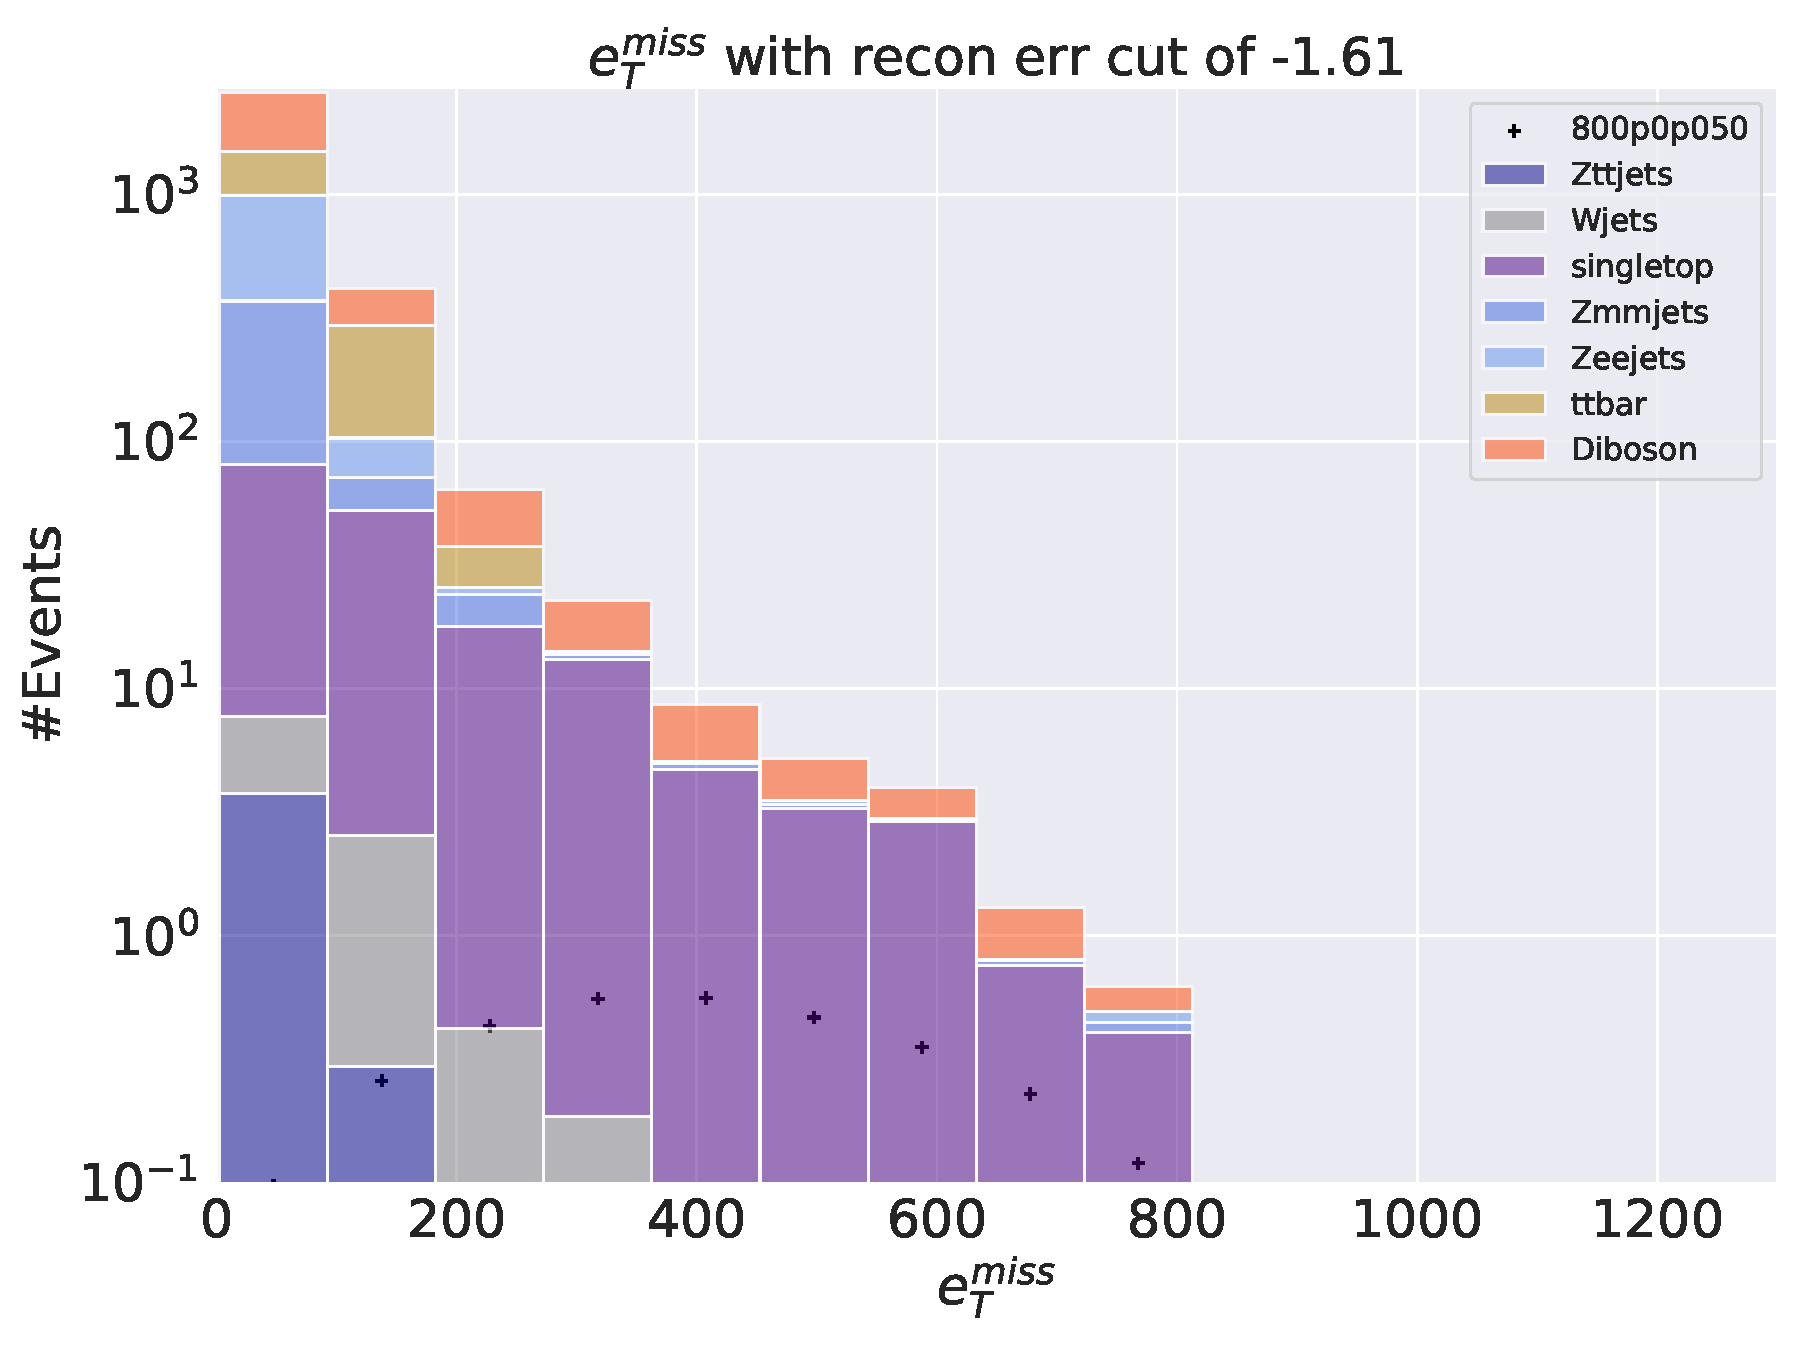
\includegraphics[width=\textwidth]{Figures/AE_testing/small/2lep/b_data_recon_big_rm3_feats_sig_800p0p050_recon_errcut_-1.61.pdf}
        \caption{}
        \label{fig:AE_2lep_small_800_cut_etmiss}
    \end{subfigure}
    \hfill      
    \caption[$e_T^{miss}$ best cuts for regular autoencoder]{$e_T^{miss}$ distribution for small (left) and large (right) autoencoder 
    . Figures \ref{fig:AE_2lep_big_450} and \ref{fig:AE_2lep_small_450} shows the SUSY 450 and 300 mass signal, 
    and figures \ref{fig:AE_2lep_big_800} and \ref{fig:AE_2lep_small_800} shows the SUSY 800 and 50 mass signal.}
    \label{fig:AE_2lep_recon_err_both_sig_cut_etmiss}
\end{figure}
